\section{Analysis and Characterization of Main Memory Accesses in DNN}
\label{sec:char}
%We analyze and characterize main memory accesses in DNN and use the analysis results to drive our design.
We characterize main memory accesses in DNN to drive our design.


\subsection{Profiling Framework}
\label{sec:profiling_framework}
%The major profiling challenge is to semantic difference between OS (page) and app (tensors)


We build a profiling framework for our study.
The profiling framework collects the following information: the number of \textit{main memory accesses} per data object (tensor), data object size and lifetime. 

To collect the above information, the profiling framework includes the support at \textit{both} OS and TensorFlow runtime levels. At the OS level, \name collects the number of memory accesses at the page level. This is implemented by a software-only solution. In particular, when a page is tracked for access counting, \name sets a reserved bit (bit 51) in its PTE (i.e., poisoning PTE) and then flush the PTE from TLB. When the page is accessed, a TLB miss occurs and triggers a protection fault. \name uses a customized fault handler to count this page access, poison the PTE and flush it from TLB again to track next page access. Poisoning PTE and flushing TLB only happens during the profiling. %After it, poisoning PTE and flushing TLB do not happen. 


%\textcolor{red}{poisoning PTEs at the page table(i.e., setting PTE reserved bit) and then flushing the PTE from TLB. When the page be accessed again, a TLB miss occurs and triggers a protection fault. \name implement customized TLB miss handler to record page access information and poison this PTE again to keep recording the next of this page access. Note that \name profiling triggers a customized system call to start collect the number of memory access at page level. When the profiling finishes, another system call will be triggered and PTEs will no longer be poisoned. }

%To bridge the semantic gap between OS and application, each memory page has only one data object (but a data object can use more than one pages). 
To bridge the semantic gap between OS and application, each memory page has only one data object (but a data object can use more than one pages). \textcolor{check}{This is implemented by making object allocation aligned with memory page.} Using this method, page-level profiling becomes data object-level profiling. Such memory allocation does not change memory access patterns captured by the hardware caching mechanism in the cache hierarchy, hence providing reliable estimation on main memory accesses. %Such memory allocation only slightly increases memory footprint (discussed in Section~\ref{sec:eval_results}). But it happens during the profiling phase of \name on slow memory.
It only slightly increases memory footprint (discussed in Section~\ref{sec:eval_results}) and happens during the profiling phase of \name on slow memory.
After the profiling phase, data objects are re-organized to reduce memory footprint and improve performance. Data reorganization happens \textit{during memory allocation} (see Section~\ref{sec:profiling_results}), and hence does not stop training process and does not impact performance. Also, the profiling method does not increase the consumption of fast memory. 


At the TensorFlow runtime level, \name leverages memory allocation and deallocation to get the size and lifetime of data objects. Furthermore, \name introduces an API that allows the user to annotate DNN to indicate the end of each layer in DNN.
%Furthermore, \name introduces two APIs that allow the user to annotate DNN to indicate the start and end of each layer in DNN. 
Based on the above infrastructure, \name is able to associate a data object with the DNN topology (i.e., we can know which layer(s) a data object is alive), 
which is helpful to direct data migration (Section~\ref{sec:adaptive_dm}). 
%.Setting up the association is helpful to direct data migration (Section~\ref{sec:adaptive_dm}). 

%%%%%%%%%%adding the reason for profiling at the OS level
\textcolor{check}{The above profiling method is featured with the coordination between OS and TensorFlow runtime. Such a method provides accurate profiling, which is unachievable by TensorFlow runtime alone. In particular, OS allows us to track memory accesses filtered by processor caches; Working with the coordination between OS and TensorFlow runtime, we do not need to handle pointer aliasing commonly found in TensorFlow implementation, which is difficult to be handled by a runtime solution. It is possible that we use \texttt{mprotect()} at the application level to track memory accesses to each data object without changing OS. However, given a large number of data objects, we have to extensively change TensorFlow implementation to apply \texttt{mprotect()}, which is not practical.}


%%%%\textcolor{jie}{
%%%The profiling framework involves OS level instead of only using application level data objects information because of following reason. 
%%%%Profiling at both OS level and application level is the optimal solution to get data object access information for DNN training workload because of following reasons. First, profiling at OS level can eliminates processor cache effect and obtain more accuracy result for page-based memory management. Second, profiling memory access in application level for DNN training workload is not trivial.  Frameworks(e.g., TensorFlow) and mathematical libraries(e.g., NumPy~\cite{oliphant2006guide}) for DNN training implemented with large amount of memory pointers and no runtime memory management(i.e., implemented by C/C++). Therefore, application level profiling needs large amount of pointer arithmetic to get the memory address where data objects access happens. Existing work~\cite{madt} explores profiling page access in user-space by using \textit{mprotect()} POSIX system call. However, DNN training workload involves large amount of data objects and each of them needs to make the system call to track page access, which is not practical.}

%%%%%%%%%%%%%%%%

Our profiling method uses only one training step for profiling. During the profiling, \name captures each page read and write by repeatedly poisoning the page. This is expensive because of system calls and TLB misses. However, it does not lose profiling accuracy. Also, considering that a typical DNN training involves millions of training steps, the profiling overhead is easily amortized.  The traditional profiling methods face a %fundamental 
dilemma between profiling overhead and accuracy. In particular, frequently collecting memory access information brings high profiling accuracy at the cost of large runtime overhead, and vice versa~\cite{Thermostat:asplos17,RAMinate:socc16,heteros:isca17, sc18:wu, unimem:sc17}. Leveraging the repetitiveness of DNN training, \name breaks the dilemma, and enables both high profiling accuracy and low profiling overhead. 

%\textcolor{green}{paragraph: Existing work use OS level profile use sampling based approach intercept TLB miss to capture hot and code pages.}

%\textcolor{green}{paragraph: TensorFlow provides profiling API to profile the input and output tensor for operations. The information is course-gained and not suitable for migration: (1) lack of tensor access info which has been used instead of operations. (not work for short-lived tensor). (2) lack of tensor location information. tensorflow profiling API only provide the information of the pointer points to tensor instead of the real address of tensors. The pointer information is not suitable for page migration. }

%\textcolor{green}{paragraph: app level profiling: profiling tensor access in app runtime ask for a lot of engineering efforts. need to intercept every tensor access in every operation. Not practical, not general.}

%\textcolor{green}{paragraph: Our profiling method. We adopt the combination of profiling in both OS level and app level. In app level we intercept tensor allocator/deallocator to get tensor size and lifetime information; In OS level we poison PTE to trigger protection fault and record every page access.}

%\textcolor{green}{paragraph: Due to the predicative of ML model, profiling one training step without sampling can have more accurate result. Profiling happens on slow memory.

%\subsection{Profiling Results and Analysis}
\subsection{\textcolor{dong2}{Observations and Preliminary Analysis}}
\label{sec:profiling_results}

\begin{comment}
\begin{figure}[!t]
\centering
%\vspace{-10pt}
%\includegraphics[width=0.48\textwidth]{ASPLOS2020_Jie/figures/f1_3edit.pdf}
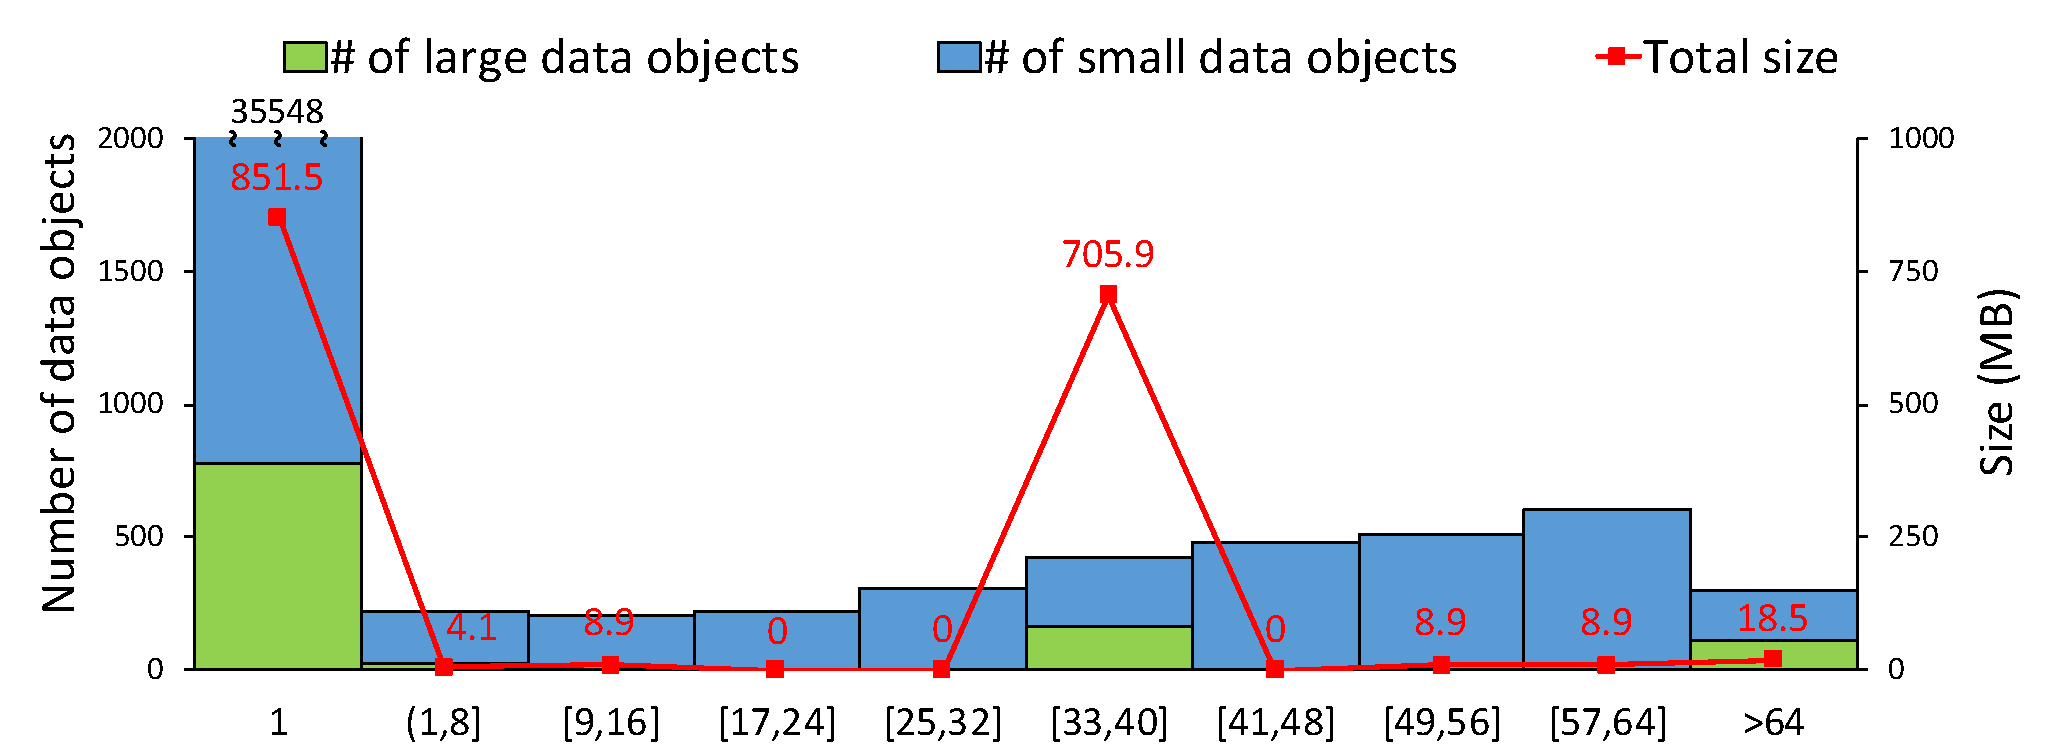
\includegraphics[width=0.48\textwidth]{figures/figure1.pdf}
%\vspace{-10pt}
%\caption{\name tensor access histogram.  x-axis shows tensor access frequency and y-axis shows the number of tensors.}
\caption{Distribution of lifetime of data objects and their sizes for ResNet\_v1-32. Each small data object is smaller than 4KB; Each large data object is no smaller than 4KB. ``>64'' means that the data object survives more than one forward and backward pass (one training step).}
%\textcolor{red}{need to conform}}
%\vspace{-10pt}
\label{fig:fig_lifetime}
\end{figure}

We use the profiling framework to study data objects and their access patterns in DNN. We report profiling results for one training step in this section.


\end{comment}

We profile DNN models listed in Table~\ref{tab:models} \textcolor{dong2}{and come up with the following observations, which guide our design: }

\textbf{Observation 1}: There are a large number of small data objects with short lifetime in DNN training workloads.

\textcolor{check}{
A data object is alive after it is allocated and before it is freed. We define the lifetime of a data object in terms of the number of layers where the data object is alive. In the rest of the paper, we define short-lived data objects as those whose lifetime is no longer than one layer. Taking ResNet-32 as an example (the configuration is in Table~\ref{tab:models}), 92\% of its data objects have lifetime no longer than one layer. Among them, 98\% is small data objects (smaller than 4KB). The peak memory consumption of short-lived data objects is small, and typically bounded by a few GB.}

%Figure~\ref{fig:fig_lifetime} shows the distribution of lifetime of data objects and their accumulated sizes for ResNet\_v1-32 (the configuration of training is in Table~\ref{tab:models}). ResNet\_v1-32 has 64 layers (in a forward and backward pass). A data object is alive after it is allocated and before it is freed. The lifetime of a data object is defined in terms of number of layers where the data object is alive. Figure~\ref{fig:fig_lifetime} shows that 92\% of data objects have lifetime no longer than one layer. Among those short-lived data objects, 98\% of them is small data objects (smaller than 4KB). 


\begin{comment}
\begin{figure}[!t]
\centering
%\vspace{-5pt}
%\includegraphics[width=0.48\textwidth]{figures/tensor_access.pdf}
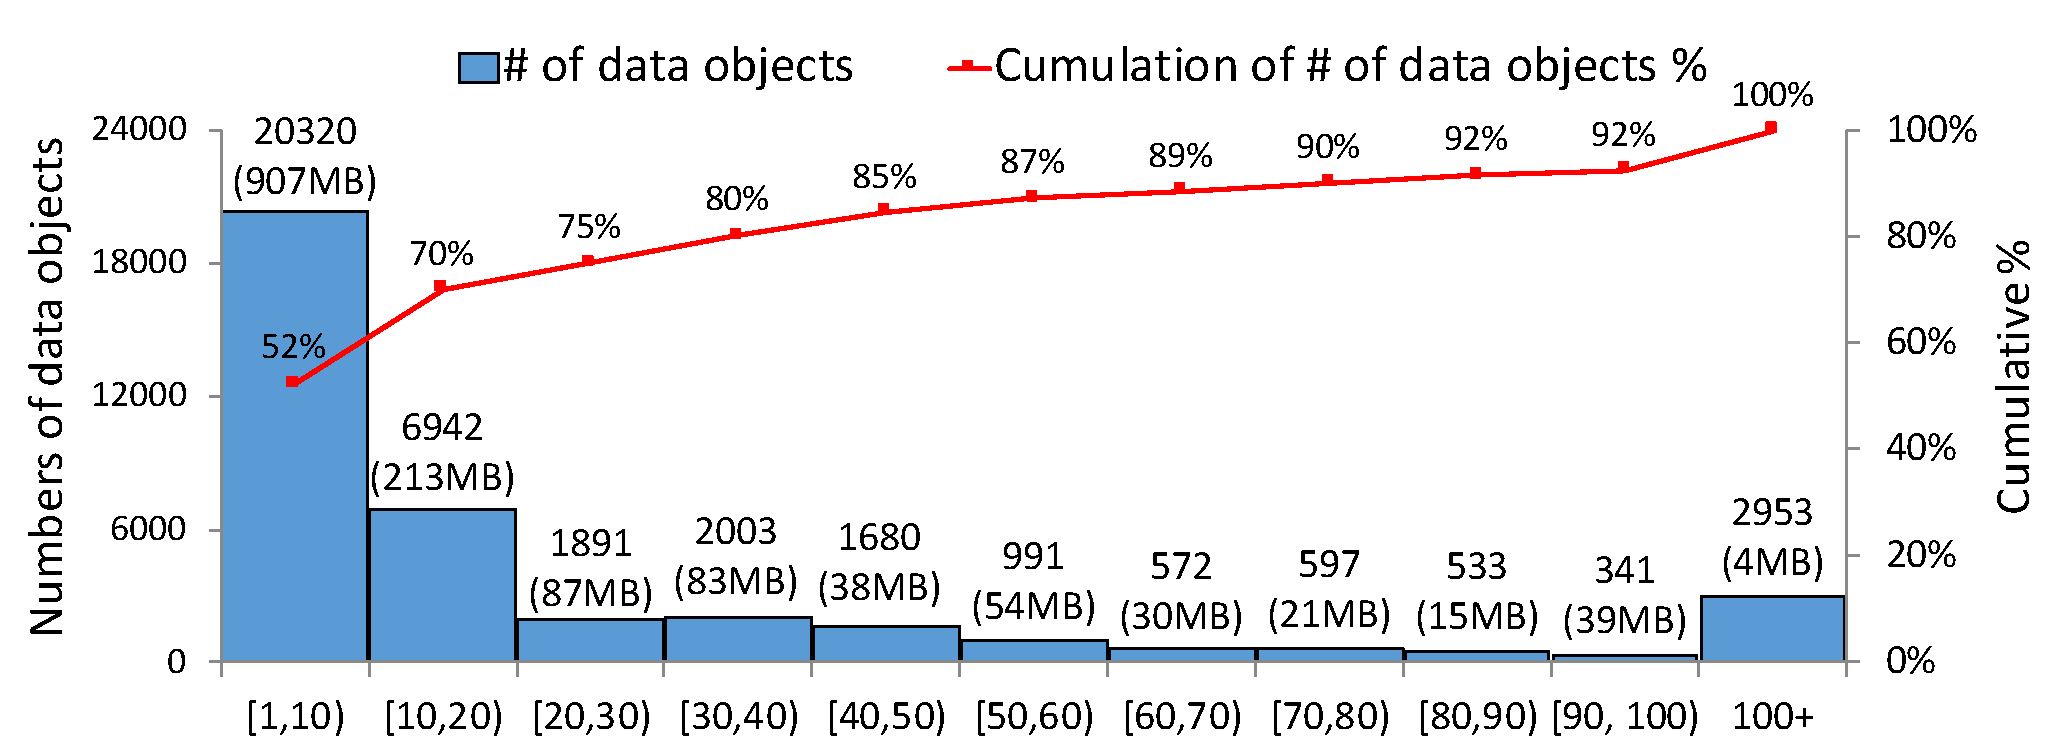
\includegraphics[width=0.48\textwidth]{figures/figure2.pdf}
%\vspace{-20pt}
%\caption{\name tensor access histogram.  x-axis shows tensor access frequency and y-axis shows the number of tensors.}
\caption{Distribution of the number of main memory accesses at the data object level.}
%\vspace{-5pt}
\label{fig:tensor_access}
\end{figure}

\begin{figure}[!t]
\centering
%\vspace{-20pt}
%\includegraphics[width=0.48\textwidth]{figures/small_tensor_access.pdf}
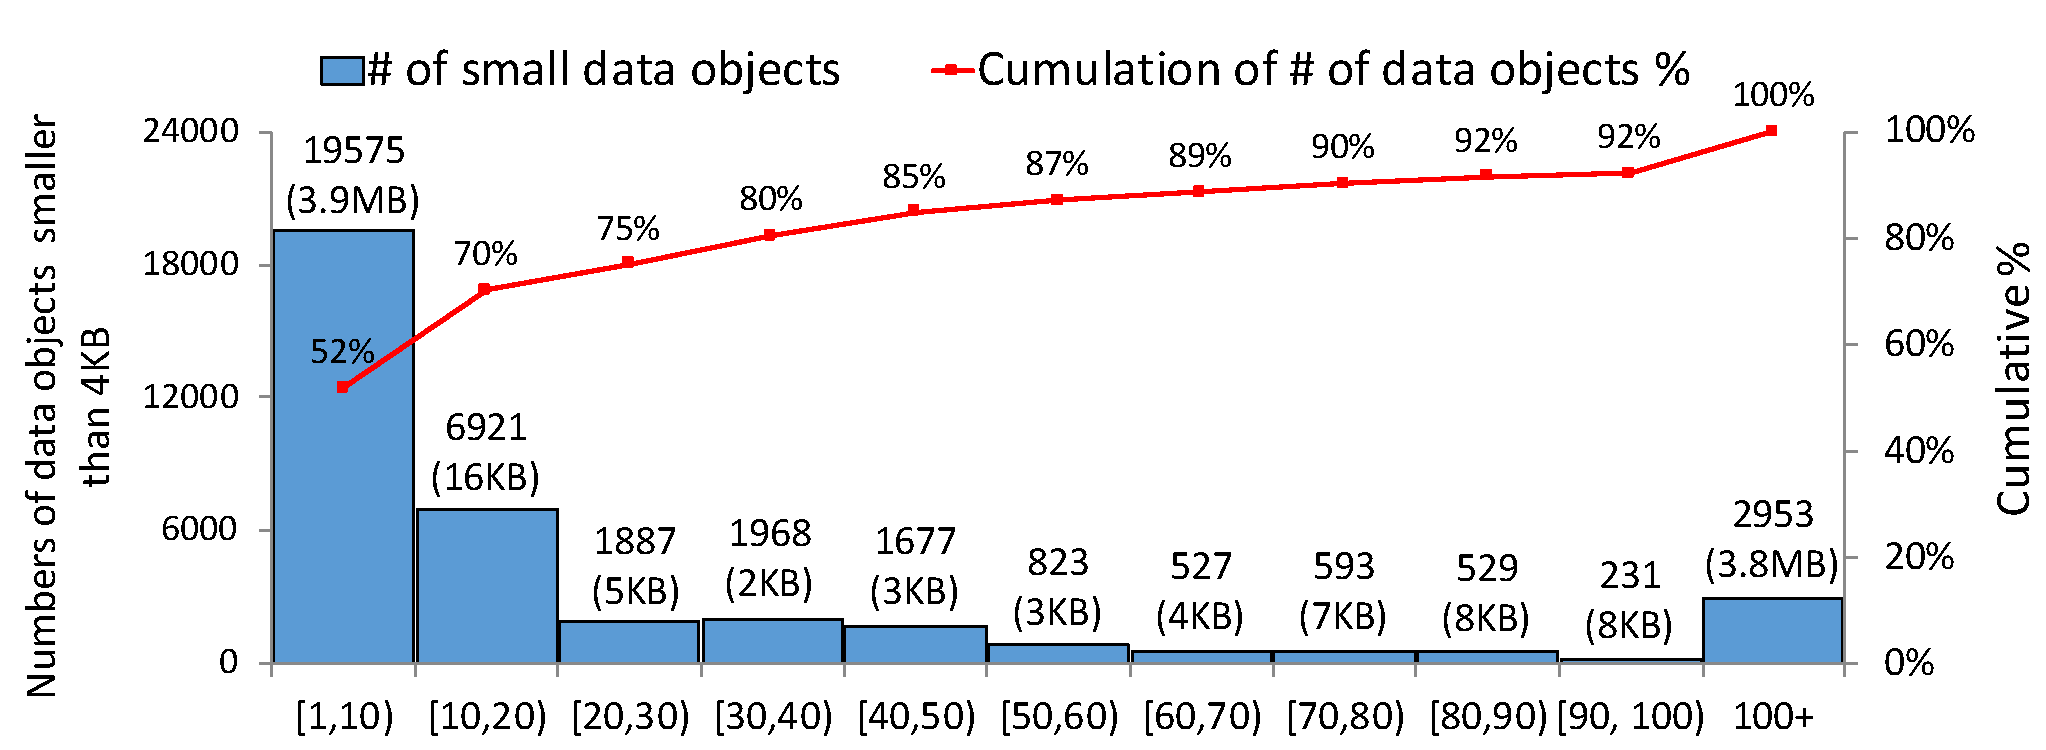
\includegraphics[width=0.48\textwidth]{figures/figure3.pdf}
%\vspace{-25pt}
%\caption{\name tensor access histogram.  x-axis shows tensor access frequency and y-axis shows the number of tensors.}
\caption{Distribution of the number of main memory accesses at the data object level for small data objects (each is smaller than 4KB).}
%\vspace{-10pt}
\label{fig:small_tensor_access}
\end{figure}
\end{comment}


\textbf{Observation 2}: The uneven distribution of hot and cold data objects provides opportunities for data management. 

\textcolor{check}{
%Use ResNet-32 as an example again. 
52.3\% of data objects (using 907 MB, which is 54\% of total memory pages) in ResNet-32 are accessed less than 10 times in main memory. On the other hand, some data objects in ResNet-32 are frequently accessed (having >100 accesses), taking only 4 MB (0.2\% of total memory pages). They are the candidates to be placed into fast memory, and their size is a small portion of total memory pages. }


\begin{comment}
Figure~\ref{fig:tensor_access} shows the distribution of the number of main memory accesses at the data object level. 
%We collect the data in the figure after data re-organization. 
%%%\textcolor{green}{We collect the data in figure by allocating each memory page has only one data object.}
The figure shows that a large number of data objects (52.3\% of data objects, using 907 MB, which is 54\% of total memory pages) are accessed less than 10 times. Among them, 98\% of them are small (\textcolor{dong2}{less than 4KB}) and use only 3.9 MB in total, shown in Figure~\ref{fig:small_tensor_access}. On the other hand, some data objects are frequently accessed (having >100 accesses), taking only 4 MB (0.2\% of total memory pages). They are the candidates to be placed into fast memory, and their size is a small portion of total memory pages. 

\begin{figure}[!t]
\centering
%\vspace{-20pt}
\includegraphics[width=0.48\textwidth]{figures/tensor_access.pdf}
%\vspace{-20pt}
%\caption{\name tensor access histogram.  x-axis shows tensor access frequency and y-axis shows the number of tensors.}
\caption{Distribution of the number of main memory accesses at the data object level.}
%\vspace{-5pt}
\label{fig:tensor_access}
\end{figure}

\begin{figure}[!t]
\centering
%\vspace{-20pt}
\includegraphics[width=0.48\textwidth]{figures/small_tensor_access.pdf}
%\vspace{-25pt}
%\caption{\name tensor access histogram.  x-axis shows tensor access frequency and y-axis shows the number of tensors.}
\caption{Distribution of the number of main memory accesses at the data object level for small data objects (each is smaller than 4KB).}
%\vspace{-10pt}
\label{fig:small_tensor_access}
\end{figure}
\end{comment}


\textbf{Observation 3}: Page-level false sharing exists in DNN. The page-level profiling (not data object-level) for data management can be misleading. 

\textcolor{check}{In ResNet-32, if we perform data object-level profiling, we find that in a training step, for those less-frequently accessed data objects that have only 1-10 accesses in main memory, their total object size is 907 MB. However, if we perform page-level profiling, we find that in the same training step, for those memory pages with 1-10 accesses in main memory, their total page size is 763 MB.  This indicates that some less-frequently accessed data objects fall into some pages that are counted as more frequently accessed. Hence, if one uses page-level profiling to guide data management, those less-frequently accessed data objects can be placed into fast memory and waste memory space and bandwidth. We refer to the above result as page-level false sharing. }


\begin{comment}
\begin{table}[!tbh]
%\vspace{-10pt}
%\small
\centering
\caption{Memory consumption (in one training step) in the original execution and using ``one data object per page'' in the profiling step. ``prof.'' stands for ``profiling''.} 
\label{tab:mem_consume}
\begin{tabular}{|c|c|c|}
\hline
memory consumption                                                       & in prof. & Orig. exe.  \\ \hline
all data objects                                                         & 1.97 GB   & 1.57 GB    \\ \hline
\begin{tabular}[c]{@{}c@{}}data objects \\ smaller than 4KB\end{tabular} & 152 MB    & 0.45 MB    \\ \hline
\end{tabular}
\end{table}


Table~\ref{tab:mem_consume} shows memory consumption for two cases: (1) the original execution and (2) using ``one data object per page'' in the profiling step. In the original execution, small data objects takes only 0.45MB, but using one data object per page, they take 152 MB. This indicates that small data objects commonly share pages with other data objects. 

Figure~\ref{fig:size_diff} shows the distribution of the number of main memory accesses at different levels, including at the data object level already shown in Figures~\ref{fig:tensor_access} and~\ref{fig:small_tensor_access}, and page level in the original execution. The figure shows that for less frequently accessed data objects (having 1-10 accesses), the total size of data objects (907 MB) is larger than the total page size (763 MB) in the original execution. 

This result is interesting, because if alive data objects fall into the same pages, the size of the data objects should be smaller than or equal to the size of pages.  
%\textcolor{green}{if data objects with similar access time falling into the same pages, the size of the data objects should be smaller than or equal to the size of pages. }
Our result is against the above rationale, which suggests that some data objects actually do not fall into those 763MB-pages in the original execution. This means in the original execution, those data objects fall into other pages that are counted as more frequently accessed. In other words, those data objects share the pages with other data objects that may have different preference for data placement. We refer to the above result as \textit{page-level false sharing} in the rest of the paper. 
\end{comment}



%This indicates that some of these data objects are placed into the same page. Since the data objects in the same page can be accessed at different execution time, such a memory page can be . An example of this case is xxxx. We call this case page-level false sharing in the rest of the paper.




%%We notice that 48\% of pages is not frequently accessed (less than ten times). %Those pages have great potential to be placed in slow memory in most of the training time. Those frequently accessed pages (having >500 accesses) only take about \textcolor{red}{xxx} MB (3.3\% of total memory pages). This result is different from Figure~\ref{fig:tensor_access} at the tensor level. page-level false sharing.
%Those hot pages are candidates to be placed into fast memory. The small size of those hot pages shows great potential to use a small fast memory.

\begin{comment}
\begin{figure}
\centering
%\vspace{-20pt}
\includegraphics[width=0.48\textwidth]{figures/page_access.pdf}
%\vspace{-25pt}
\caption{Distribution of the number of main memory accesses at the page level without data re-organization.}
%\caption{x-axis shows the page access frequency and the y-axis shows the number of pages.}
%\vspace{-10pt}
\label{fig:page_access}
\end{figure}

%\textcolor{red}{Figure: show the number of tensors and their sizes per layer. Purpose of this figure: to show the variance of tensor usages across layers.}

\begin{figure}[!th]
\centering
%\vspace{-20pt}
%\includegraphics[width=0.48\textwidth]{figures/mem_size.pdf}
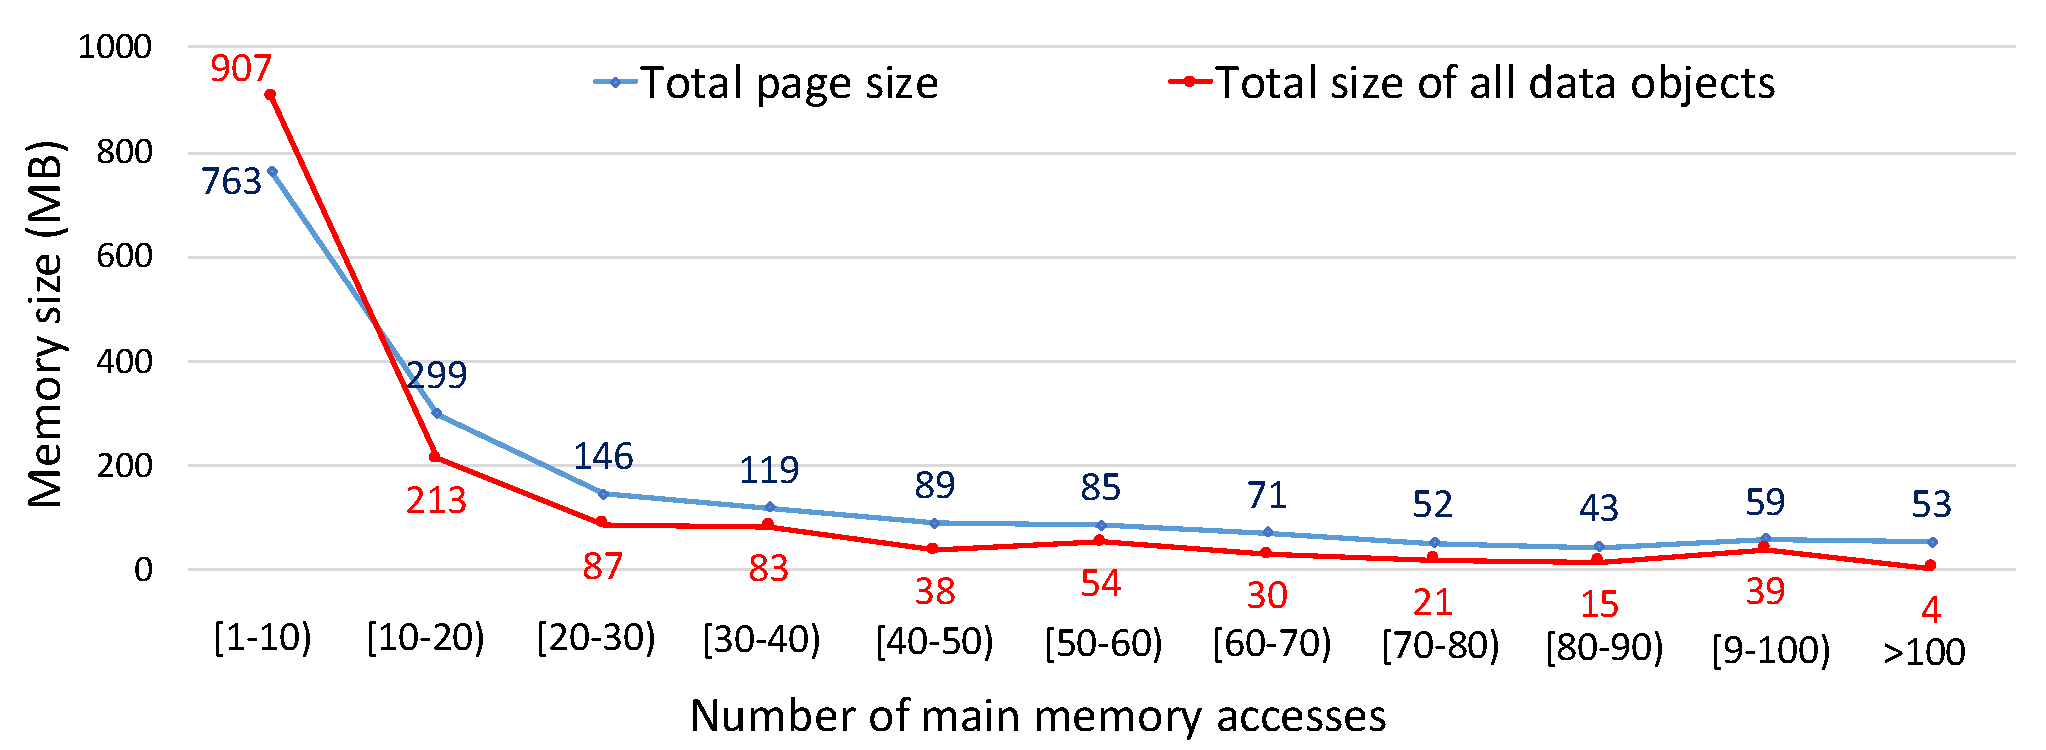
\includegraphics[width=0.48\textwidth]{figures/figure4.pdf}
%\vspace{-25pt}
%\caption{\name tensor access histogram.  x-axis shows tensor access frequency and y-axis shows the number of tensors.}
\caption{Distribution of the number of main memory accesses at the levels of pages (in the original execution), data objects, and small data objects.}
%\vspace{-10pt}
\label{fig:size_diff}
\end{figure}
\end{comment}


%\textcolor{green}{Figure~\ref{fig:page_access} shows main memory page access distribution in page level. More than 50\% of pages access time is less 10 times. Figure~\ref{fig:size_diff} shows the accumulated size with different profiling method. Page-level profiling can over-estimate data object access because of false-sharing.}



%%%%%%%%%%%%%%%%%%%%%new example
\begin{figure}
\centering
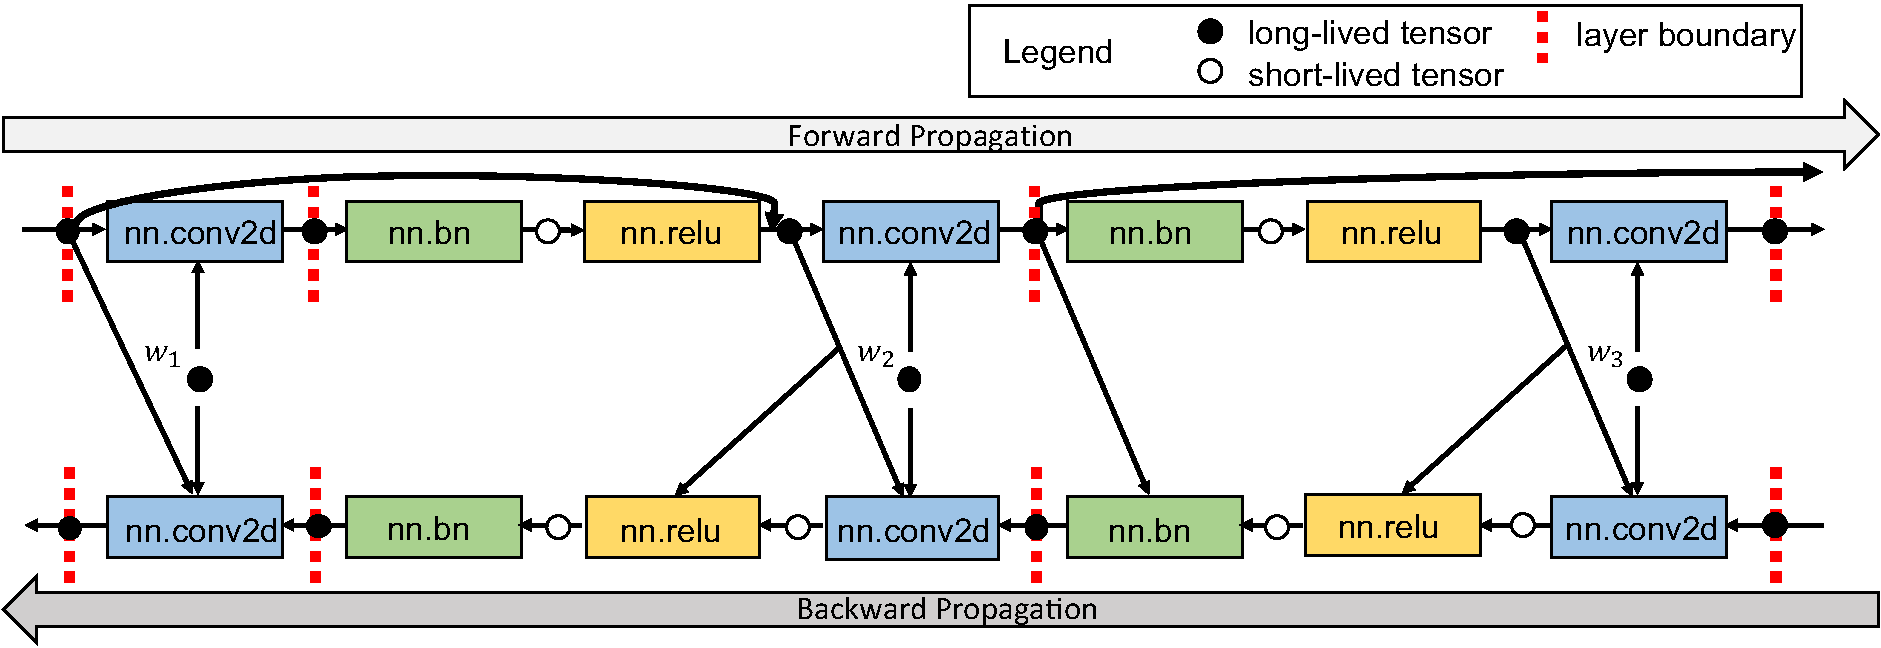
\includegraphics[width=0.49\textwidth]{figures/tensor_usage.pdf}
\vspace{-20pt}
\caption{\textcolor{check}{An example to show tensor access patterns across layers in ResNet-32. This figure shows the first three layers and the last three layers in ResNet-32}.}
\vspace{-5pt}
\label{fig:tensor_usage}
\end{figure}
\begin{figure}
\centering
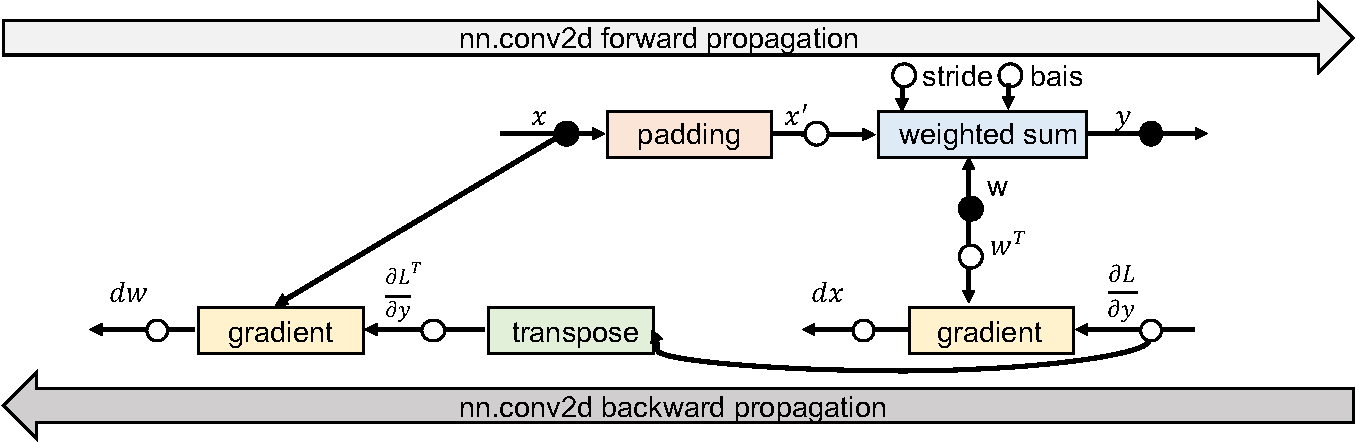
\includegraphics[width=0.48\textwidth]{figures/conv_tensor_usage.pdf}
\vspace{-20pt}
\caption{\textcolor{check}{Data processing in a TensorFlow operation, \texttt{nn.conv2d}.}}
\vspace{-10pt}
\label{fig:conv_tensor_usage}
\end{figure}


\textcolor{check}{
\textbf{Example.} %We discuss observations in the context of a DNN model (ResNet-32) 
\textcolor{dong2}{To see more details, let us use an example of ResNet-32 }
to understand how data objects are managed in a typical DNN workload. Figure~\ref{fig:tensor_usage} shows operations in six layers, and Figure~\ref{fig:conv_tensor_usage} shows data processing in a common operation (\texttt{nn.conv2d}) used in forward and backward propagation of DNN. }

\textcolor{check}{\textit{Long-lived tensors.} We find two cases. (1) Weights associated with each layer (shown as ``w1'' and ``w2'' etc. in Figure~\ref{fig:tensor_usage}). They are allocated before training steps, and updated throughout them.  (2) Intermediate results generated in a layer and consumed by the downstream operations in another layers. An example is the output tensors of operations \texttt{nn.conv2d} and \texttt{nn.relu} in the forward propagation layers shown in Figure~\ref{fig:conv_tensor_usage}. These output tensors are consumed %by the backward propagation layers. 
\textcolor{dong2}{by the backward propagation layers to calculate gradients.}
The memory space for these intermediate results is allocated when they are generated and then freed after they are consumed.}


\begin{comment}
\textcolor{check}{\textit{Short-lived tensors.}
We find three cases. (1) Inside an operation, many data processing (e.g., padding and transpose shown in Figure~\ref{fig:conv_tensor_usage}, expansion, concatenation and squeeze) generates short-lived tensors, which are only used in that operation; (2) The output tensor of some operation is short-lived, exemplified by the output of batch normalization (i.e.,\textit{nn.bn} in Figure~\ref{fig:tensor_usage}); (3) Some tensors generated but never consumed in a DNN model. These tensors are generated, in order to enable operation generality across various DNN models. The gradient of input $dx$ in \texttt{nn.conv2d} backward propagation in Figure~\ref{fig:conv_tensor_usage} is such an example.  Memory allocation and free for a short-lived tensor always happen in one layer.}
\end{comment}

\textcolor{check}{\textit{Short-lived tensors.}
We find two cases. (1) Inside an operation, many data processing (e.g., padding and transpose shown in Figure~\ref{fig:conv_tensor_usage}, expansion, concatenation and squeeze) generates short-lived tensors, which are only used in that operation; (2) The output tensor of some operation is short-lived, exemplified by the output of batch normalization (i.e.,\textit{nn.bn} in Figure~\ref{fig:tensor_usage}). Memory allocation and free for a short-lived tensor always happen in one layer.}

\textit{Memory access patterns.}
Memory accesses to all tensors are associated with layers. Memory accesses to a long-lived tensor tend to be \textcolor{dong2}{\textit{``sparse''} and \textit{periodical}}, which means memory accesses happen in a couple of specific layers, but not all layers. Memory accesses to short-lived tensors tends to be \textcolor{dong2}{\textit{ephemeral} and \textit{bursty},} which means
in a layer, there can be a number of short-lived tensors created, accessed a few times, and freed. In addition, memory allocations for long-lived  intermediate results and short-lived tensors are interleaved throughout the training process, which creates opportunities for page-level false sharing.


%There are a large number of short-lived data objects during the DNN training and not accessed many times (Observation 1). For one operation, the intermediate results and the output are allocated memory before the operation execution and might share the same memory page. However, those data objects have different access patterns(Observation 3). Without data object management in DNN training, the short-lived data objects and the long-lived data objects can be allocated in the same memory pages, which makes the memory usage inefficient. 



\begin{comment}
\textcolor{jie}{
\textbf{Example. }
%%%%\name treats forward and backward pass into different layers. Data object in different layer has different reuse.
We use an example to explain memory access in DNN training.
%Computation graph declaration and execution are separated in DNN training framework. 
%For example, TensorFlow codes contains two parts, graph building and session running. 
%Data objects keep allocating and deallocating during computation graph execution. 
Figure~\ref{fig:tensor_usage} illustrates data objects access in ResNet~\cite{resnet_32}. 
Operations consume data objects produced by previous operations and calculate outputs. 
The outputs of convolution (i.e., \textit{nn.conv2d}) and ReLU(i.e., \textit{nn.relu}) participate calculation in future layers, and they are long-lived data objects; while the outputs of batch normalization(i.e.,\textit{nn.bn}) are only used in the same layer and they are identified as short-lived data objects. The memory access for data objects are not evenly distributed. For example, the outputs of ReLU have more memory access than the outputs of convolution(Observation 2). 
}
\end{comment}

%\textcolor{jie}{Further, we analysis data objects access within an operation. Figure~\ref{fig:conv_tensor_usage} shows the data object access of \textit{nn.conv2d} operation in TensorFlow. Instead of each operation, there are large amounts of data objects for intermediate results. In figure~\ref{fig:conv_tensor_usage}, the memory for output of padding and transpose are allocated before the convolution begins and deallocated after the convolution finished.  The intermediate results are common after calculations like padding, transpose, expansion, concatenation and squeeze, and they are all short-lived. Instead of the intermediate result, the outputs of operation may also be a short-lived tensor. As shown in figure~\ref{fig:conv_tensor_usage}, there are two outputs for the convolution operation in backward propagation, the gradient of weights \textit{dw} and the gradient of input \textit{dx}.  \textit{dx} is not used in later computation in ResNet while it is still calculated and its memory is allocated because of the generality of the training framework. There are a large number of short-lived data objects during the DNN training and not accessed many times (Observation 1). For one operation, the intermediate results and the output are allocated memory before the operation execution and might share the same memory page. However, those data objects have different access patterns(Observation 3). Without data object management in DNN training, the short-lived data objects and the long-lived data objects can be allocated in the same memory pages, which makes the memory usage inefficient. }

\textcolor{check}{\textbf{Design choices.} Profiling results motivate us to make three design choices. (1) We choose DNN layer as the basic granularity for data management, given the fact that lifetime and memory access patterns of data objects are associated with layers. This choice brings convenience for data prefetching and migration overhead controlling. (2) We treat data objects differently, instead of using a unified, application-agnostic policy to manage them as in~\cite{Yan:ASPLOS19, unimem:sc17, sc18:wu}. This choice allows us to enable high performance and minimize fast memory capacity. (3) We do not use static analysis as in~\cite{pldi19:panthera} to decide data placement, because static analysis lacks timing information needed to overlap data migration and computation; It cannot accurately capture main memory accesses and ignores the impact of thread-level parallelism on data locality.}
%It is difficult for static analysis to identify data objects because of pointer aliasing.




%\textcolor{jie}{\textbf{Design Choices.} Large amounts of data objects with various of size, lifetime, and access patterns make data management for DNN training challenging. The goal of \name is to narrow down the performance difference between HM and fast memory only system. To achieve this, \name tries the best effort to make data objects happens in fast memory as much as possible. The different characteristics of data objects make \name treats them differently. \name reallocates data objects according to their characteristics to make memory usage efficiently (discuss in section~\ref{sec:dyn_profiling_data_org}). Short-lived data objects are not suitable for migration, and \name handles it separately (discuss in section~\ref{sec:short-lived}). For long-live data objects, \name migrates them proactively according to profiling results (discuss in section~\ref{sec:adaptive_dm}).  However, static analysis is not enough for \name to make data placement and migration decision because (1) the short-lived data objects within operations can not be captured by static analysis, and (2) static analysis can not obtain memory access in DNN training. \name provides a data management solution for DNN training without the knowledge of DNN model implemented details.}